\chapter{Aromaticité et substitution électrophile aromatique}\label{ch:b2:aromatic-substitution}

L'eau de brome se décolore en quelques secondes quand on l'agite avec un alcène, et pas du tout
avec le benzène. Pourtant, le benzène réagit bien avec le dibrome dès qu'on ajoute un peu de
bromure de fer(III) --- et le produit, le bromobenzène, possède encore son cycle \omterm{def:b2:huckel:aromatic}{aromatique} à
six atomes~: un hydrogène a été remplacé, rien n'a été ajouté. Les cycles \omterm{def:b2:huckel:aromatic}{aromatiques} subissent
des substitutions plutôt que des additions, parce qu'une addition sacrifierait la stabilisation
calculée au \cref{ch:b2:huckel}. Le même mécanisme nitre, sulfone, alkyle et acyle les cycles
benzéniques, et les groupes déjà présents sur un cycle décident, avec une régularité surprenante,
de la position du suivant.

\begin{recall}
\Cref{ch:b2:huckel}~: l'aromaticité et l'\omterm{def:b2:huckel:delocalisation}{énergie de délocalisation} du benzène. Le volume de
première année~: additions électrophiles sur les alcènes, effets inductif et mésomère, groupes
donneurs et accepteurs, carbocations et leurs réarrangements, postulat de Hammond, acides de Lewis,
profils énergétiques.
\end{recall}

\begin{omfigure}
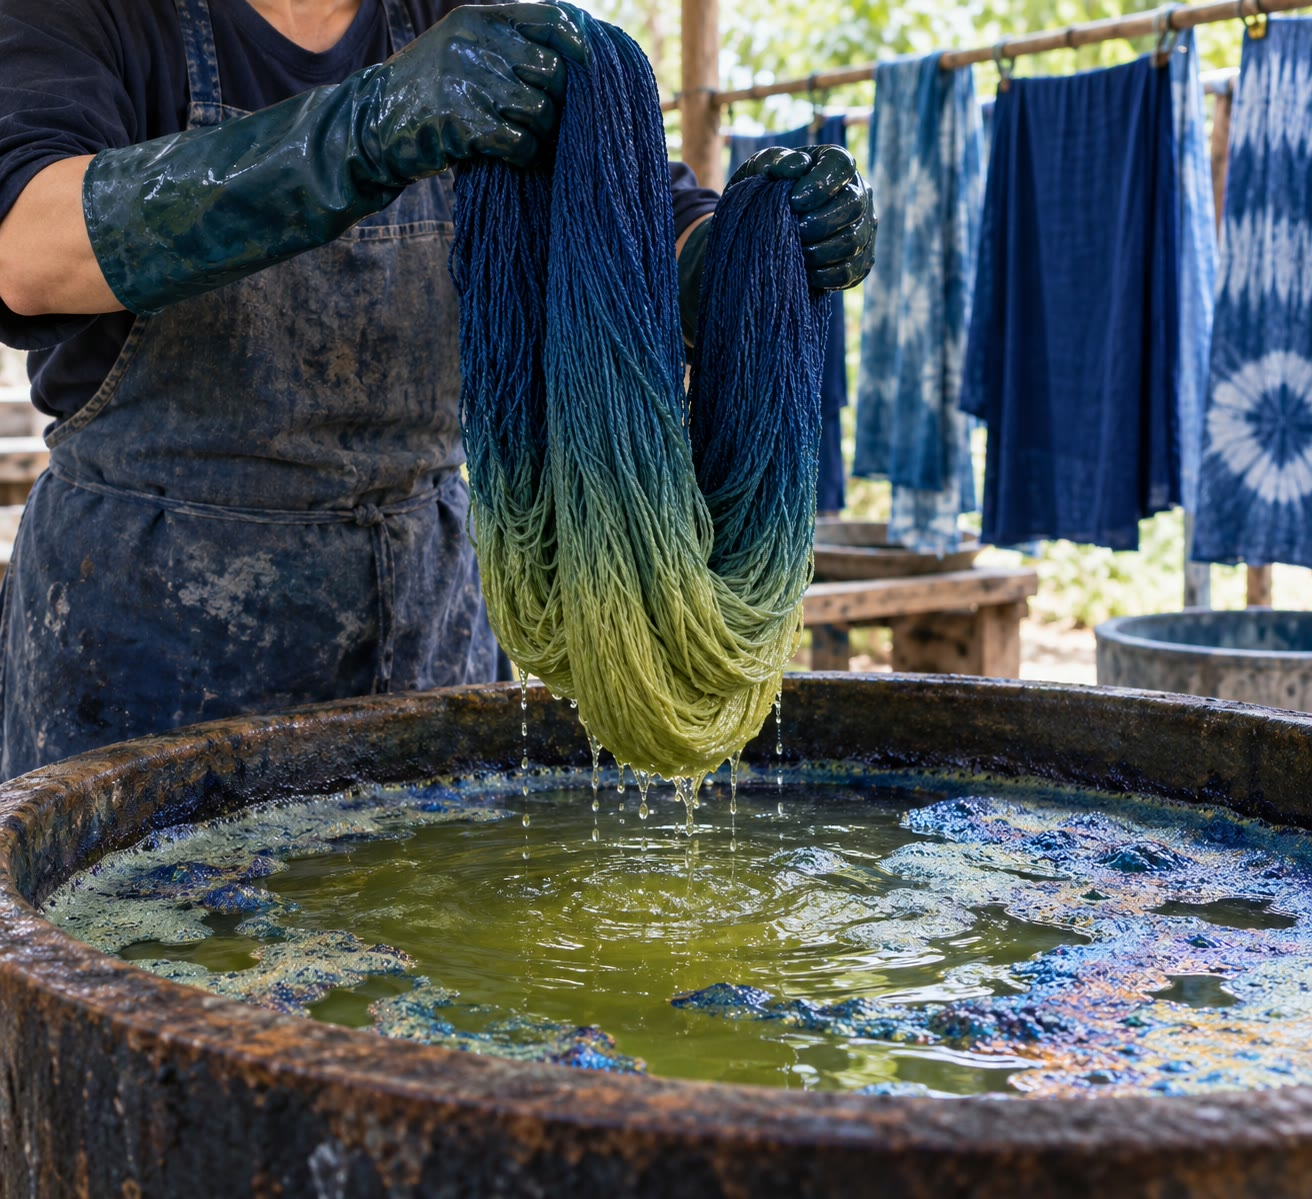
\includegraphics[width=0.55\linewidth]{images/book3/ai/b2-22-indigo-vat-2.jpg}

{\small Teinture de fils dans une cuve d'indigo (illustration). Le fil sort de la cuve jaune-vert,
imprégné de la forme réduite et soluble du colorant, et bleuit à l'air quand le dioxygène le
retransforme en indigo insoluble. L'indigo, comme la plupart des colorants, est construit sur des
cycles \omterm{def:b2:huckel:aromatic}{aromatiques}~; l'industrie des colorants du \textsc{xix}\textsuperscript{e}~siècle est née
des réactions de substitution de ce chapitre appliquées au benzène tiré du goudron de houille.}
\end{omfigure}

\section{Substitution et non addition}

\begin{definition}[Arène]\label{def:b2:aromatic-substitution:arene}
Un \emph{arène}\index{arene@arène} est un hydrocarbure contenant au moins un cycle \omterm{def:b2:huckel:aromatic}{aromatique},
comme le benzène, le toluène (méthylbenzène) ou le naphtalène~; un groupe aryle (\ce{Ar}) est un
arène privé d'un hydrogène.
\end{definition}

\begin{proposition}[Pourquoi le benzène ne s'additionne pas]\label{prop:b2:aromatic-substitution:no-addition}
Une addition sur le benzène transformerait le cycle \omterm{def:b2:huckel:aromatic}{aromatique} en un cyclohexadiène non \omterm{def:b2:huckel:aromatic}{aromatique}
et ferait perdre l'essentiel des \qty{150}{kJ/mol} de stabilisation \omterm{def:b2:huckel:aromatic}{aromatique}~; la substitution la conserve.
\end{proposition}

\begin{proof}[Argument]
Au \cref{ch:b2:huckel}, l'hydrogénation du benzène en cyclohexa-1,3-diène s'est révélée
\omterm{def:b2:reaction-enthalpy:exothermic}{endothermique} (\qty{+22}{kJ/mol}, à partir de \qty{-206.0}{} et \qty{-227.7}{kJ/mol}), alors que
celle d'une double liaison ordinaire libère \qty{119}{kJ/mol}~: la première addition est l'étape
coûteuse. Après la première étape électrophile, le cation formé peut soit fixer un nucléophile,
ce qui laisse un \omterm{def:b2:frontier-orbitals:diels-alder}{diène} non \omterm{def:b2:huckel:aromatic}{aromatique}, soit perdre un proton, ce qui restaure le cycle \omterm{def:b2:huckel:aromatic}{aromatique}.
La seconde voie est de loin la plus favorable.
% ledger: dfh:C6H6_g, dfh:C6H8_g, dfh:C6H10_g, dfh:C6H12_g
\end{proof}

\section{Le mécanisme}

\begin{definition}[Substitution électrophile aromatique]\label{def:b2:aromatic-substitution:seAr}
Une \emph{substitution électrophile aromatique}\index{substitution electrophile aromatique@substitution électrophile aromatique}
remplace un hydrogène d'un cycle \omterm{def:b2:huckel:aromatic}{aromatique} par un électrophile \ce{E+}. L'électrophile se lie
d'abord à un carbone du cycle, ce qui donne un cation dans lequel ce carbone est tétraédrique et
la charge positive est répartie sur les cinq autres~: l'\emph{intermédiaire de Wheland}\index{intermediaire de Wheland@intermédiaire de Wheland}
(un ion arénium). Une base arrache ensuite le proton du carbone tétraédrique.
\end{definition}

\begin{proposition}[Deux étapes]\label{prop:b2:aromatic-substitution:mechanism}
La première étape, qui détruit l'aromaticité, est l'étape lente~; la perte du proton, qui la
restaure, est rapide.
\end{proposition}

\begin{proof}[Argument]
L'\omterm{def:b2:aromatic-substitution:seAr}{intermédiaire de Wheland} est un carbocation stabilisé par délocalisation sur trois carbones,
mais non \omterm{def:b2:huckel:aromatic}{aromatique}~: il se situe bien au-dessus des réactifs et, d'après le postulat de Hammond,
l'état de transition qui y conduit lui est proche en structure et en énergie. La seconde étape
descend vers un produit \omterm{def:b2:huckel:aromatic}{aromatique}~: sa barrière est faible.
\end{proof}

\begin{omfigure}
\begin{tikzpicture}
\begin{axis}[width=0.55\linewidth, height=5.4cm, xmin=-0.2, xmax=4.2, ymin=-5.5, ymax=11.5,
  axis x line=bottom, axis y line=left, xtick=\empty, ytick=\empty,
  xlabel={coordonnée de réaction}, ylabel={énergie}, label style={font=\small}, clip=false]
\addplot[omDef, thick] table[x=x, y=sub] {figdata/out/bachelor-2-aromatic-profile.dat};
\addplot[omThm, thick, dashed, restrict x to domain=2:4] table[x=x, y=add] {figdata/out/bachelor-2-aromatic-profile.dat};
\node[font=\scriptsize, anchor=north west] at (axis cs:0.0,-0.6) {\ce{ArH + E+}};
\node[font=\scriptsize, anchor=north] at (axis cs:2,5.7) {Wheland};
\node[font=\scriptsize, anchor=west, omDef] at (axis cs:4.05,-4.0) {\ce{ArE + H+}};
\node[font=\scriptsize, anchor=west, omThm] at (axis cs:4.05,2.0) {produit d'addition};
\node[font=\scriptsize, anchor=south] at (axis cs:1,10.1) {lente};
\end{axis}
\end{tikzpicture}

{\small Profil énergétique d'une \omterm{def:b2:aromatic-substitution:seAr}{substitution électrophile aromatique}, schématique (un modèle).
La première étape, qui forme l'\omterm{def:b2:aromatic-substitution:seAr}{intermédiaire de Wheland}, a la barrière la plus haute. La perte
d'un proton (trait plein) restaure le cycle \omterm{def:b2:huckel:aromatic}{aromatique}~; la fixation d'un nucléophile (tirets)
laisserait un produit situé au-dessus des réactifs.}
\end{omfigure}

\begin{omfigure}
\setchemfig{atom sep=2em}
\schemestart
\chemfig{HO-\chemabove{N}{\scriptstyle +}(=[1]O)-[7]\chemabove{O}{\scriptstyle -}} \+ \chemfig{H_2SO_4}
\arrow{<=>}
\chemfig{O=N^{+}=O} \+ \chemfig{HSO_4^{-}} \+ \chemfig{H_2O}
\schemestop

\medskip
\begin{tikzpicture}[font=\small, >={Stealth}]
\tikzset{pics/whel/.style n args={4}{code={
    \foreach \k in {0,...,5} \draw[thick] ({90+60*\k}:0.7) -- ({150+60*\k}:0.7);
    \foreach \k in {#1} \draw[thick] ($({90+60*\k}:0.56)!0.18!({150+60*\k}:0.56)$) -- ($({90+60*\k}:0.56)!0.82!({150+60*\k}:0.56)$);
    \ifnum#2>-1 \node[font=\scriptsize] at ({90+60*#2}:0.36) {$+$};\fi
    \draw[thick] (270:0.7) -- ++(-125:0.42) node[anchor=north east, inner sep=1pt, font=\scriptsize] {H};
    \draw[thick] (270:0.7) -- ++(-55:0.42) node[anchor=north west, inner sep=1pt, font=\scriptsize] {#4};
    \if\relax\detokenize{#3}\relax\else
      \draw[thick] (90:0.7) -- (90:1.1) node[anchor=south, inner sep=1pt, font=\scriptsize] {#3};\fi
  }}}
  \foreach \k in {0,...,5} \draw[thick] ({90+60*\k}:0.7) -- ({150+60*\k}:0.7);
  \foreach \k in {0,2,4} \draw[thick] ($({90+60*\k}:0.56)!0.18!({150+60*\k}:0.56)$) -- ($({90+60*\k}:0.56)!0.82!({150+60*\k}:0.56)$);
  \node at (1.3,0) {$+$};
  \node at (2.0,0) {\ce{NO2+}};
  \draw[->, thick] (2.6,0) -- (3.8,0) node[midway, above, font=\scriptsize] {lente};
  \pic at (4.7,0.1) {whel={1,4}{0}{}{\ce{NO2}}};
  \draw[->, thick] (5.6,0) -- (6.8,0) node[midway, above, font=\scriptsize] {rapide} node[midway, below, font=\scriptsize] {$-$\ce{H+}};
  \begin{scope}[xshift=7.7cm]
    \foreach \k in {0,...,5} \draw[thick] ({90+60*\k}:0.7) -- ({150+60*\k}:0.7);
    \foreach \k in {0,2,4} \draw[thick] ($({90+60*\k}:0.56)!0.18!({150+60*\k}:0.56)$) -- ($({90+60*\k}:0.56)!0.82!({150+60*\k}:0.56)$);
    \draw[thick] (270:0.7) -- (270:1.1) node[anchor=north, font=\scriptsize] {\ce{NO2}};
  \end{scope}
\end{tikzpicture}
\par\vspace{6pt}

{\small Nitration du benzène. L'acide sulfurique protone l'acide nitrique, qui perd de l'eau~:
l'ion nitronium \ce{NO2+} est l'électrophile. Il se lie à un carbone (étape lente), ce qui donne
l'\omterm{def:b2:aromatic-substitution:seAr}{intermédiaire de Wheland}, dont la charge positive est répartie sur le cycle~; la perte d'un
proton (étape rapide) donne le nitrobenzène.}
\end{omfigure}

\section{Les réactions}

\paragraph{Halogénation.} Le dibrome ou le dichlore seul est un électrophile trop faible~; un acide
de Lewis (\ce{FeBr3}, \ce{AlCl3}) polarise l'halogène en se liant à l'un de ses atomes, et l'atome
de brome externe attaque le cycle.

\paragraph{Nitration.} Un mélange d'acides nitrique et sulfurique concentrés (ci-dessus) fournit
l'ion nitronium.

\paragraph{Sulfonation.} L'oléum (\ce{SO3} dans \ce{H2SO4}) donne l'acide benzènesulfonique.
La réaction est renversable~: chauffer l'acide sulfonique en solution aqueuse acide diluée retire
de nouveau le groupe \ce{SO3H}, ce qui en fait un groupe bloquant temporaire utile.

\begin{definition}[Réactions de Friedel--Crafts]\label{def:b2:aromatic-substitution:friedel-crafts}
Une \emph{alkylation de Friedel--Crafts}\index{alkylation de Friedel--Crafts} fixe un groupe
alkyle sur un cycle \omterm{def:b2:huckel:aromatic}{aromatique} à partir d'un halogénoalcane et d'un acide de Lewis (\ce{AlCl3}). Une
\emph{acylation de Friedel--Crafts}\index{acylation de Friedel--Crafts} fixe un groupe acyle
\ce{RCO} à partir d'un chlorure d'acyle et de \ce{AlCl3}, par l'intermédiaire de l'\emph{ion acylium}\index{ion acylium}
\ce{R-C#O+}, et donne une cétone \omterm{def:b2:huckel:aromatic}{aromatique}.
\end{definition}

\begin{proposition}[Limites des réactions de Friedel--Crafts]\label{prop:b2:aromatic-substitution:friedel-crafts-limits}
L'\omterm{def:b2:aromatic-substitution:friedel-crafts}{alkylation de Friedel--Crafts} souffre des réarrangements du carbocation et de la
polyalkylation~; l'acylation s'arrête après une substitution, ne donne aucun réarrangement et
exige au moins un équivalent de \ce{AlCl3}. Ni l'une ni l'autre ne fonctionne sur un cycle
portant un groupe fortement désactivant.
\end{proposition}

\begin{proof}[Argument]
L'électrophile alkylant est un carbocation (ou un complexe polarisé qui se comporte comme tel),
qui se réarrange en un carbocation plus stable par migration d'hydrure ou d'alkyle~: le
1-chloropropane donne surtout de l'isopropylbenzène. Un groupe alkyle active le cycle (section
suivante), si bien que le produit réagit plus vite que le benzène et s'alkyle de nouveau. L'\omterm{def:b2:aromatic-substitution:friedel-crafts}{ion
acylium} est stabilisé par résonance (\ce{R-C+=O} $\leftrightarrow$ \ce{R-C#O+}) et ne se
réarrange pas~; le groupe acyle désactive le cycle, si bien que le produit ne réagit pas
davantage~; enfin la cétone formée fixe \ce{AlCl3} par son oxygène, ce qui retire le catalyseur
du milieu~: un équivalent est consommé. Un cycle fortement désactivé est un nucléophile trop
pauvre pour ces électrophiles faibles.
\end{proof}

\section{Effets des substituants}

\begin{definition}[Groupes orienteurs]\label{def:b2:aromatic-substitution:directing}
Un substituant d'un cycle benzénique est un \emph{groupe activant}\index{groupe activant} si le
cycle réagit plus vite que le benzène, un \emph{groupe désactivant}\index{groupe desactivant@groupe désactivant} s'il
réagit plus lentement. C'est un \emph{orienteur ortho/para}\index{orienteur ortho/para} si le
nouveau groupe entre principalement aux positions voisines et à la position opposée, un
\emph{orienteur méta}\index{orienteur meta@orienteur méta} s'il entre principalement aux positions
séparées de lui par un carbone.
\end{definition}

\begin{proposition}[Donneurs et accepteurs]\label{prop:b2:aromatic-substitution:directing}
Les groupes qui cèdent des électrons au cycle par effet mésomère (\ce{-OH}, \ce{-OCH3}, \ce{-NH2},
\ce{-NHCOCH3}) ou par effet inductif et \omterm{def:b2:fragment-orbitals:hyperconjugation}{hyperconjugaison} (alkyles) activent le cycle et orientent
en ortho/para. Les groupes qui attirent les électrons par effet mésomère (\ce{-NO2}, \ce{-CN}, \ce{-COR},
\ce{-COOH}, \ce{-SO3H}) le désactivent et orientent en méta.
\end{proposition}

\begin{proof}
Comparer les \omterm{def:b2:aromatic-substitution:seAr}{intermédiaires de Wheland}. Pour une attaque en ortho ou en para d'un substituant G,
l'une des trois formes mésomères place la charge positive sur le carbone qui porte G~; pour une
attaque en méta, aucune. Un donneur G (un doublet non liant sur O ou N) stabilise une charge
positive sur le carbone auquel il est lié, en ajoutant une quatrième forme mésomère dans laquelle
chaque atome possède un octet~: les intermédiaires ortho et para sont abaissés et, d'après le
postulat de Hammond, les états de transition qui y mènent aussi. Un accepteur G déstabilise une
charge positive sur son carbone~: les intermédiaires ortho et para sont élevés, et l'attaque en
méta, qui évite cette forme, est la moins défavorisée, bien que plus lente que sur le benzène.
\end{proof}

\begin{omfigure}
\begin{tikzpicture}[font=\small]
\tikzset{pics/whel/.style n args={4}{code={
    \foreach \k in {0,...,5} \draw[thick] ({90+60*\k}:0.7) -- ({150+60*\k}:0.7);
    \foreach \k in {#1} \draw[thick] ($({90+60*\k}:0.56)!0.18!({150+60*\k}:0.56)$) -- ($({90+60*\k}:0.56)!0.82!({150+60*\k}:0.56)$);
    \ifnum#2>-1 \node[font=\scriptsize] at ({90+60*#2}:0.36) {$+$};\fi
    \draw[thick] (270:0.7) -- ++(-125:0.42) node[anchor=north east, inner sep=1pt, font=\scriptsize] {H};
    \draw[thick] (270:0.7) -- ++(-55:0.42) node[anchor=north west, inner sep=1pt, font=\scriptsize] {#4};
    \if\relax\detokenize{#3}\relax\else
      \draw[thick] (90:0.7) -- (90:1.1) node[anchor=south, inner sep=1pt, font=\scriptsize] {#3};\fi
  }}}
  \node[anchor=east] at (-1.0,0) {méthoxy, attaque en para~:};
  \pic at (0,0) {whel={1,4}{0}{\ce{OCH3}}{E}};
  \node at (1.25,0.1) {$\leftrightarrow$};
  \begin{scope}[xshift=2.5cm]
    \foreach \k in {0,...,5} \draw[thick] ({90+60*\k}:0.7) -- ({150+60*\k}:0.7);
    \foreach \k in {1,4} \draw[thick] ($({90+60*\k}:0.56)!0.18!({150+60*\k}:0.56)$) -- ($({90+60*\k}:0.56)!0.82!({150+60*\k}:0.56)$);
    \draw[thick] (-0.06,0.7) -- (-0.06,1.1); \draw[thick] (0.06,0.7) -- (0.06,1.1);
    \node[anchor=south, inner sep=1pt, font=\scriptsize] at (0,1.1) {$\overset{+}{\mathrm O}\mathrm{CH_3}$};
    \draw[thick] (270:0.7) -- ++(-125:0.42) node[anchor=north east, inner sep=1pt, font=\scriptsize] {H};
    \draw[thick] (270:0.7) -- ++(-55:0.42) node[anchor=north west, inner sep=1pt, font=\scriptsize] {E};
  \end{scope}
  \node[anchor=west, font=\scriptsize] at (3.4,0) {forme de plus, chaque atome à l'octet};
  \begin{scope}[yshift=-3.5cm]
    \node[anchor=east] at (-1.0,0) {nitro, attaque en para~:};
    \pic at (0,0) {whel={1,4}{0}{\ce{NO2}}{E}};
    \node[anchor=west, font=\scriptsize] at (1.0,0) {charge positive sur le carbone porteur de l'accepteur};
  \end{scope}
\end{tikzpicture}

{\small \omterm{def:b2:aromatic-substitution:seAr}{Intermédiaires de Wheland} pour une attaque en para d'un substituant. Avec le méthoxy, un
doublet non liant de l'oxygène partage la charge positive (une forme mésomère supplémentaire, tous
les atomes à l'octet)~: l'intermédiaire est stabilisé, le substituant est activant et \omterm{def:b2:aromatic-substitution:directing}{orienteur
ortho/para}. Avec le nitro, une forme place la charge positive sur le carbone qui porte le groupe
attracteur d'électrons~: l'intermédiaire est déstabilisé, et l'attaque se fait en méta.}
\end{omfigure}

\begin{proposition}[Halogènes]\label{prop:b2:aromatic-substitution:halogens}
Les substituants halogénés désactivent le cycle mais orientent en ortho/para.
\end{proposition}

\begin{proof}[Argument]
Leur effet inductif attracteur (électronégativité) abaisse la densité électronique de tout le
cycle et ralentit toutes les attaques~: ils sont désactivants. Mais un doublet non liant de
l'halogène peut encore partager la charge positive des \omterm{def:b2:aromatic-substitution:seAr}{intermédiaires de Wheland} ortho et para,
ce dont l'intermédiaire méta ne peut profiter~: parmi les attaques ralenties, l'ortho et le para
restent les moins lentes.
\end{proof}

\section{Benzènes polysubstitués}

\begin{method}[Prévoir la position de substitution]\label{met:b2:aromatic-substitution:predict-position}
\begin{enumerate}
  \item Pour chaque substituant, repérer les positions qu'il favorise (ortho/para ou méta).
  \item S'ils concordent, cette position l'emporte. S'ils divergent, l'activant le plus fort décide
        (\ce{-NH2}, \ce{-OH} $>$ \ce{-OCH3} $>$ \ce{-NHCOCH3} $>$ alkyle $>$ halogène).
  \item Éviter la position située entre deux substituants en relation 1,3 (encombrée), et
        attendre le para plutôt que l'ortho quand les groupes sont volumineux.
\end{enumerate}
\end{method}

\begin{method}[Planifier une synthèse aromatique]\label{met:b2:aromatic-substitution:plan-aromatic}
\begin{enumerate}
  \item Choisir l'ordre des étapes de sorte que chaque groupe déjà présent oriente le suivant
        là où on le veut~: pour préparer le 3-bromonitrobenzène, nitrer d'abord (\omterm{def:b2:aromatic-substitution:directing}{orienteur méta}),
        puis bromer~; pour préparer le 4-bromonitrobenzène, bromer d'abord.
  \item Utiliser des groupes convertibles~: un groupe acyle (méta) peut être réduit en alkyle
        (ortho/para)~; un groupe nitro (méta) réduit en amine (ortho/para)~; un alkyle oxydé en
        \ce{-COOH} (méta).
  \item Bloquer une position par \ce{-SO3H} et retirer ce groupe à la fin.
  \item Modérer un activant fort~: une amine est acylée (\ce{-NHCOCH3}) avant une nitration ou
        une halogénation, puis libérée de nouveau.
\end{enumerate}
\end{method}

\begin{history}[Friedel et Crafts]
\begin{minipage}[t]{0.18\linewidth}
\vspace{0pt}
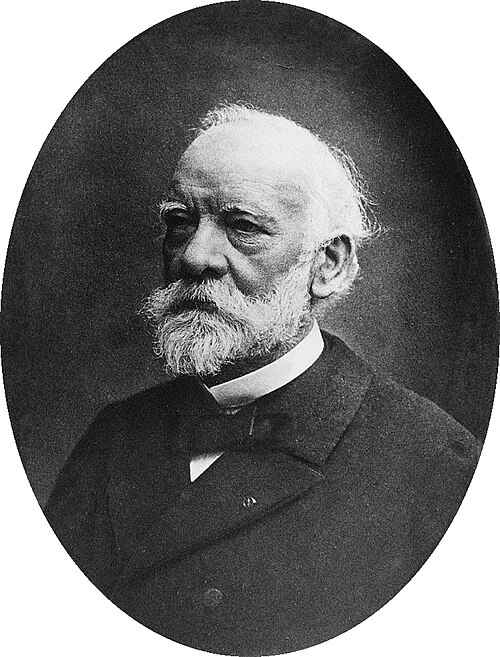
\includegraphics[width=\linewidth]{images/book3/friedel.jpg}
\end{minipage}\hspace{0.02\linewidth}%
\begin{minipage}[t]{0.18\linewidth}
\vspace{0pt}
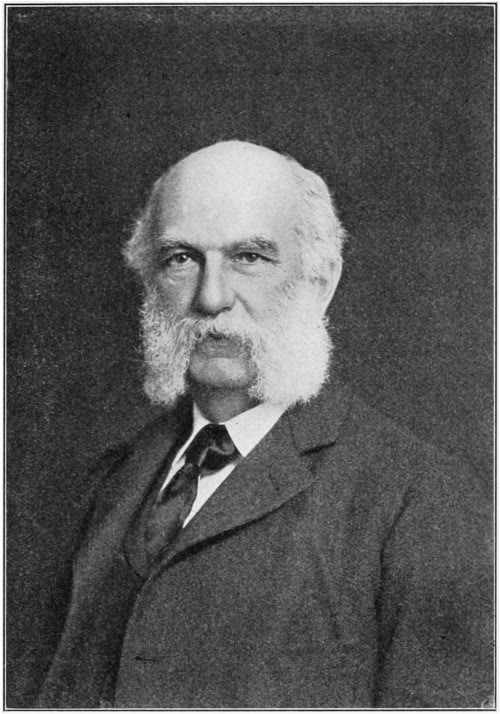
\includegraphics[width=\linewidth]{images/book3/crafts.jpg}
\end{minipage}\hfill
\begin{minipage}[t]{0.58\linewidth}
\vspace{0pt}
En 1877, Charles Friedel et James Mason Crafts, qui travaillaient ensemble à Paris, découvrirent
que le chlorure d'aluminium fait réagir les halogénoalcanes et les chlorures d'acyle avec le
benzène. Leurs réactions devinrent la méthode courante pour fixer des groupes carbonés sur les
cycles \omterm{def:b2:huckel:aromatic}{aromatiques}, et la catalyse par les acides de Lewis qu'ils avaient découverte alla bien
au-delà. (Portraits~: Friedel, années 1890~; Crafts, d'après
\textit{Popular Science Monthly}, 1900~; domaine public, Wikimedia Commons.)
\end{minipage}
\end{history}

\begin{safety}{\ghs[5mm]{GHS02}\,\ghs[5mm]{GHS05}\,\ghs[5mm]{GHS06}\,\ghs[5mm]{GHS08}}
Le benzène est cancérogène et on le remplace par le toluène ou d'autres \omterm{def:b2:aromatic-substitution:arene}{arènes} chaque fois que
possible. Les acides nitrique et sulfurique concentrés sont corrosifs et le mélange nitrant est
fortement oxydant~; on le refroidit et on ajoute l'\omterm{def:b2:aromatic-substitution:arene}{arène} lentement, car les nitrations sont
\omterm{def:b2:reaction-enthalpy:exothermic}{exothermiques}. Le dibrome est très toxique et corrosif~; le chlorure d'aluminium réagit
violemment avec l'eau. Les nitroarènes sont toxiques.
% ledger: ghs:benzene, ghs:toluene, ghs:HNO3, ghs:H2SO4, ghs:Br2, ghs:AlCl3, ghs:nitrotoluene-4
\end{safety}

\section{Exercices}

\begin{exercise}[$\star$]\label{exo:b2:aromatic-substitution:1}
Écrire la formation de l'ion nitronium à partir de l'acide nitrique et de l'acide sulfurique.
\end{exercise}

\begin{exercise}[$\star$]\label{exo:b2:aromatic-substitution:2}
Donner les produits principaux de la bromation (\ce{Br2}, \ce{FeBr3}) du toluène et du
nitrobenzène.
\end{exercise}

\begin{exercise}[$\star$]\label{exo:b2:aromatic-substitution:3}
Classer en activant ou désactivant, \omterm{def:b2:aromatic-substitution:directing}{orienteur ortho/para} ou méta~: \ce{-CH3}, \ce{-OH}, \ce{-Cl},
\ce{-NO2}, \ce{-COCH3}, \ce{-NHCOCH3}.
\end{exercise}

\begin{exercise}[$\star$]\label{exo:b2:aromatic-substitution:4}
Donner le produit formé par le benzène avec le chlorure d'éthanoyle et le chlorure d'aluminium.
\end{exercise}

\begin{exercise}[$\star\star$]\label{exo:b2:aromatic-substitution:5}
Le benzène et le 1-chloropropane, en présence de \ce{AlCl3}, donnent surtout de
l'isopropylbenzène. Expliquer, et proposer une voie en deux étapes vers le propylbenzène.
\end{exercise}

\begin{exercise}[$\star\star$]\label{exo:b2:aromatic-substitution:6}
Le phénol décolore aussitôt l'eau de brome, sans catalyseur, en donnant le
2,4,6-tribromophénol. Expliquer.
\end{exercise}

\begin{exercise}[$\star\star$]\label{exo:b2:aromatic-substitution:7}
Proposer des synthèses du 3-bromonitrobenzène et du 4-bromonitrobenzène à partir du benzène.
\end{exercise}

\begin{exercise}[$\star\star$]\label{exo:b2:aromatic-substitution:8}
L'aniline se nitre mal (oxydation, et produit méta), mais l'acétanilide donne surtout le
4-nitroacétanilide. Expliquer ces deux faits.
\end{exercise}

\begin{exercise}[$\star\star$]\label{exo:b2:aromatic-substitution:9}
Montrer comment un groupe acide sulfonique permet de préparer du 2-bromotoluène exempt de son isomère para.
\end{exercise}

\begin{exercise}[$\star\star\star$]\label{exo:b2:aromatic-substitution:10}
Où le 4-méthylanisole (4-méthoxytoluène) subit-il la nitration~? Expliquer à l'aide des deux
groupes orienteurs.
\end{exercise}

\begin{exercise}[$\star\star\star$]\label{exo:b2:aromatic-substitution:11}
Le 2,4,6-trinitrotoluène est préparé par trois nitrations successives du toluène, chacune dans des
conditions plus dures. Expliquer pourquoi.
\end{exercise}

\begin{exercise}[$\star\star\star$]\label{exo:b2:aromatic-substitution:12}
Proposer une synthèse de l'acide 4-nitrobenzoïque à partir du toluène, puis de l'acide 3-nitrobenzoïque.
\end{exercise}

\section{Problème~: nitration du toluène}

\begin{problem}[{Problème du week-end --- l'ion nitronium et le mécanisme de la nitration, les
positions ortho, méta et para du toluène face au rapport statistique, la séparation des
isomères, et un bilan de matière}]
\label{pb:b2:aromatic-substitution:1}
Données~: températures de fusion~: 2-nitrotoluène \qty{-10}{\degreeCelsius}, 3-nitrotoluène
\qty{16}{\degreeCelsius}, 4-nitrotoluène \qty{52}{\degreeCelsius}. Données de l'exercice pour une opération~:
\qty{100}{g} de toluène, \omterm{def:b2:continuous-reactors:conversion}{taux de conversion} 90~\%, répartition des isomères 58~\% ortho, 4~\% méta,
38~\% para. Masses molaires (\unit{g/mol})~: C 12.011, H 1.008, N 14.007, O 15.999.
% ledger: mp:2-nitrotoluene, mp:3-nitrotoluene, mp:4-nitrotoluene, aw:C, aw:H, aw:N, aw:O

\medskip
\noindent\textbf{Partie I --- L'électrophile et le mécanisme.}
\begin{enumerate}
  \item Écrire la formation de l'ion nitronium.
  \item Représenter son schéma de Lewis et donner sa géométrie.
  \item Écrire l'attaque de \ce{NO2+} sur le toluène en para du méthyle.
  \item Représenter les trois formes mésomères de l'\omterm{def:b2:aromatic-substitution:seAr}{intermédiaire de Wheland} para.
  \item Quelle étape est cinétiquement déterminante~?
  \item Qu'est-ce qui arrache le proton lors de la seconde étape~?
\end{enumerate}

\medskip
\noindent\textbf{Partie II --- Les trois positions.}
\begin{enumerate}[resume]
  \item Combien le toluène possède-t-il de positions ortho, méta et para~?
  \item Quel rapport donnerait une attaque au hasard~?
  \item Représenter l'\omterm{def:b2:aromatic-substitution:seAr}{intermédiaire de Wheland} méta et expliquer pourquoi c'est le moins stabilisé.
  \item Comment le groupe méthyle stabilise-t-il les intermédiaires ortho et para~?
  \item Comparer le rapport observé au rapport statistique~: quelles positions sont favorisées~?
  \item Comparer le rendement par position en ortho (la moitié du pourcentage ortho) et en para.
        Proposer une raison à cette différence.
  \item Le toluène se nitre-t-il plus vite ou plus lentement que le benzène~?
\end{enumerate}

\medskip
\noindent\textbf{Partie III --- Séparation.}
\begin{enumerate}[resume]
  \item Quel isomère est solide à température ambiante~?
  \item Proposer une façon de l'isoler du mélange par refroidissement.
  \item Pourquoi la symétrie favorise-t-elle une température de fusion élevée~?
  \item Comment séparer ensuite les isomères ortho et méta~?
  \item Pourquoi ces isomères sont-ils difficiles à séparer par simple distillation~?
\end{enumerate}

\medskip
\noindent\textbf{Partie IV --- Bilan de matière.}
\begin{enumerate}[resume]
  \item Calculer la masse molaire du toluène et celle du nitrotoluène.
  \item Calculer la quantité de toluène et celle de nitrotoluène formé.
  \item Calculer les masses des trois isomères.
  \item Quelle réaction ultérieure faut-il éviter en refroidissant et en n'utilisant pas d'excès d'acide~?
  \item Comment préparer l'acide 4-nitrobenzoïque à partir de l'isomère para~?
  \item Donner la masse de 4-nitrotoluène obtenue à partir de \qty{100}{g} de toluène lors de cette opération.
\end{enumerate}
\end{problem}
